\chapter{Background}
\label{cha:LiteratureReview}

The chapter explains aspects required to fully comprehend the project's achievements alongside an evaluation of current literature and the respective gaps.

The chapter will contain the following sections:

\begin{itemize}
    \item \textbf{Project context} \\ 
    Will provide the user with the base knowledge required to understand the context and purpose of the following literature review.
    
    \item \textbf{Definition of terms}\\
    Specific definitions relevant to the literature review will initially be defined.
    
    \item \textbf{Literature Review} \\
    A review of currently available literature on relevant topics. Recommendations and research gaps will be identified and discussed.

\end{itemize}

\section{Project context}

To fully understand the literature review it is necessary to introduce and explain the base knowledge before continuing.

\subsection*{Public-key Cryptography and Key Exchange}

Asymmetric cryptography facilitates the secure encryption of messages in end-to-end encryption (E2EE), verification of digital signatures and sharing of pre-communication secrets, among others. 

The asymmetry stems from the use of "Public" and "Private" keys. The Public key is used to encrypt data that only the respective Private key can decrypt. This means the keys required to encrypt can be easily shared across insecure channels.

To construct an E2EE connection the initial stage will be a key exchange using the key types discussed previously. This is the sharing of a pre-shared secret between two verified parties, this will then be used to encrypt subsequent messages with symmetric encryption\footnote{This is due to the speed increase of symmetrical over asymmetrical encryption}. This, however, hinges on the verification of the initial parties, if one party impersonates another and gets to view the pre-shared secret all communication becomes decryptable. Therefore, the correct identification of parties is crucial to maintaining secure communication channels. The exploitation of this is known as a Man-in-the-middle (MiTM) attack. This can be bidirectional where the attacker can sit in the middle of a communication channel and decrypt all correspondence. Figure \ref{fig:mitm} contains a visual representation of this attack.

\begin{center}
    \newcommand{\tgap}{0.1cm}

\begin{center}
\begin{tikzpicture}[
	every node/.style={fill=white},
    diagram item/.style={},
    align=left
]         

\node (Router)[
    diagram item,
    label=above:Alice,
    yshift=-2cm
] {
\includegraphics[scale=\ciscoImageScale]{\cisco/workstation}};

\node (Victim)[
	diagram item,
	label=above:Bob,
	right of=Router,
	xshift=7cm
] {
\includegraphics[scale=\ciscoImageScale]{\cisco/workstation}};

\coordinate (CENTER) at ($(Victim)!0.5!(Router)$);
\node (Attacker)[
	label=below:Eve,
	below of=CENTER,
	yshift=-3.5cm
] {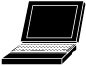
\includegraphics[scale=\ciscoImageScale]{\cisco/laptop}};

\draw[-] (Router)--node[yshift=0.5cm]{Old Connection}(Victim);
\draw[red, very thick] (Router)--node{New Connection}(Attacker);
\draw[red, very thick] (Attacker)--node{New Connection}(Victim);


\end{tikzpicture} 
\end{center}

    \begin{figure}[h]
        \caption{Photo depicting a MITM attack}
        \label{fig:mitm}
    \end{figure}
\end{center}

Due to the assumption that the attacking party (Eve) does not have the same public-private key pair as either party (Alice or Bob) the fingerprint of the public key can be used for identification. There are, however, issues in how a user should link a key's fingerprint to a real world entity. This paper will, however, assume that users have access to the respective parties' correct fingerprint, as the protocols used to achieve this are outside the project's scope.

The fingerprint of the key is generated by running the main key components through a secure one way hash function such as SHA-1. This process produces a digest of fixed length that can be used to compare keys. Therefore, the comparison of expected and actual fingerprints can be used to detect MiTM attacks.
Historically these have been represented as a hexadecimal string whereon verification fingerprints are compared between two substrates, for example, a monitor screen and a business card.
This process is known as the \textit{``authentication ceremony''}. However, system designers are moving away from this structure and are now creating a combined key from each sides' public key. In the case of WhatsApp for example, the connection fingerprint of two parties keys is the first 30 bytes of a SHA-512\footnote{5200 iterations} hash of each parties' identity key, these are then both concatenated together to form a single key\cite{whatsapp2017paper}. This produces a unique key communication pair.
\\\\
Due to the manual comparison of the fingerprint, length and format is a consideration. Prior research has shown that the average human can only hold around 7-digits worth of data in their working memory\cite{miller1956magical}. This rules out the possibility of comparing complete digests. For example, SHA-1 is 40 hex digits (160-bit) and, therefore, difficult to effectively compare. Therefore, if human interaction is required; there is a need for schemes that work effectively with consideration to individual limitations.

Research in this area has taken various encoding schemes and compared their fallibility to impersonated attacks. The main elements of comparison have been the ``accuracy of attack detection" and ``time to compare". In this paper, these are considered the metrics of ``security'' and ``usability'', respectively.

\section{Definition of terms}
Throughout the paper, various terms are used to define elements of the authentication ceremony relevant to fingerprints verification. Explicit descriptions are, therefore, stated in this section. These are used to remove ambiguity and underlying associations readers may have for the words chosen.
\\\\
\textbf{\textit{Encoding schemes}} - This is the physical method of encoding used to represent the fingerprint. For example, ``Hexadecimal'' or ``Words'' are a unique way to represent a fingerprint and thus, are encoding schemes.
\\\\
\textbf{\textit{Method of comparison}} - This is how the user assesses the encoding scheme. The most common example and the one used as default is ``Compare-and-Confirm'' (CaC). CaC, as the name suggests, is the \textit{comparison} of two fingerprints on different devices or mediums that are then \textit{confirmed}. The following sections explain alternative methods of comparisons.


\section{Literature Review}
This section will now discuss the current research around the proposed topic.

The section is organized as follows:

\begin{itemize}
    \item \textbf{Authentication ceremony performance} \\
    This section explains the current research on performance of various encoding schemes and methods of comparison. This is then complemented with an assessment of the experimentation design for the respective studies.

    \item \textbf{Encoding schemes} \\
    The following section then discusses research around the design of an encoding scheme. Focus in this section will be allocated to the technical details around the creation and design of relevant schemes. 

    \item \textbf{Attacks on encoding schemes} \\
    The final section will then discuss literature that investigates the creation of attacks against encoding schemes in order to deceive the respective users.
\end{itemize}

\subsection{Authentication ceremony performance}

\subsubsection*{Encoding scheme performance}
Results 
from the literature consistently show the effectiveness of language-based encodings such as Words or Sentences with accuracies ranging from 94\% \cite{dechand2016empirical}\cite{tan2017can}\cite{kainda2009usability}. In all cases, these were the best schemes from the sets assessed. The exception to this is the work performed by \textbf{Hsiao, \textit{et al.}}\cite{hsiao2009study} in 2009 with Words achieving an abnormal accuracy of 63.00\%.
\\\\
Aside from textual representations were graphical schemes. Examples of schemes assessed were: Random Art\cite{perrig1999hash}, Flag\cite{ellison2003public}, T-Flag\cite{lin2010spate}, Vash\footnote{https://github.com/thevash/vash}, OpenSSH visual host key and Unicorns\footnote{https://unicornify.pictures/}, among others. These schemes had mixed accuracy with ranges as large as 50\% - 94\% in work by \textbf{Hsiao, \textit{et al.}}\cite{hsiao2009study}. The only other paper assessing graphical representations was the work of \textbf{Tan \textit{et al.}}\cite{tan2017can} where they also achieved mixed results with accuracies ranging from 46\% to 90\%.
\\
\begin{table}[h!]
    \makebox[\textwidth][c]{
        \begin{tabular}{c|ccccc}
    \toprule
    \textbf{Scheme} 
    & Hsu-Chun\cite{hsiao2009study}      
    & Kainda\cite{kainda2009usability}      
    & Dechand\cite{dechand2016empirical}
    & Tan\cite{tan2017can}      
    \\\hline
    Hexadecimal     &           &           & 11.20   & 9.00\\
    Numerical       &           & 6.00      & 10.60   & 9.00\\
    Base32          & 3.51      & 6.00      & 10.20   & \\
    Words           & 4.63      & 7.00      & 8.70    & 7.00 \\
    Scentences      &           & 11.00     & 12.30   & 8.00 \\
    Chinese Symbols & 5.01   &           &         & \\
    Japanese Symbols& 5.07   &           &         & \\
    Korean Symbols  & 4.92   &           &         & \\
    \midrule
    Random Art	     & 3.21   &&&&\\
    Flag    	     & 4.28   &&&&\\
    T-Flag  	     & 4.00   &&&&\\
    Flag Ext.	     & 4.02   &&&&\\
    OpenSSH`         &&&& 5.00 &\\
    Unicorns         &&&& 3.00 &\\
    Vash             &&&& 3.00 &\\
    \bottomrule
\end{tabular}
    }%
    \caption{Timing results in seconds for the related schemes}
    \label{tab:times}
\end{table}
\\
In terms of usability of graphical schemes, the literature concurred on their high usability. The comparison speed of these schemes were all among the quickest (See Table \ref{tab:times} for an overview of timings). Other work also indirectly concurred with graphical encodings having significantly quicker comparison times compared to non-graphical schemes \cite{dechand2016empirical}\cite{kainda2009usability}.
In terms of research into the performance of graphical schemes, the literature does not contain an extensive review with literature only containing two papers. There is also no overlap in the schemes assessed with each paper reviewing a unique set. This is, therefore, a promising candidate for further research.

One unique paper in this research area was the work by \textbf{M. Shirvanian \textit{et al.}}\cite{shirvanian2017pitfalls} produced in the context of secure messaging pairing. This paper was unique for several reasons. First was to consideration for ``remote-vs-proximity'' pairing where this is the first consideration of this aspect found in the literature. There is room for further research to compare encoding schemes in the context of ``remote-vs-proximity.'' Another unique aspect was the end-to-end encryption context of the study.

The findings from the paper showed a high false negative rate for all the schemes; this is a consideration also missing from the literature. Alongside this, results for usability were lower in a remote setting for all the schemes. The author, however, comments on the expected nature of this result.\\
Images were assessed as being the most secure method of authentication in the remote setting but voted as the method with the worst usability. This conclusion is highly inconsistent with all other work in this area. However, this could be due to the unique setting of remote verification, resulting in distinct results from user studies. Without further work in this area, it is difficult to validate these results conclusively.

Alongside this, it was shown in work by \textbf{Hsiao, \textit{et al.}}\cite{hsiao2009study} that age and gender do not affect the accuracy of the scheme. However, younger participants were considerably faster. Furthermore, findings also showed that language comprehension helped in discerning small differences between schemes encoded in Chinese, Japanese, Korean or English. Subsequently, knowledge of the language did not assist in differentiating more significant changes in the schemes as these had high accuracy regardless. These were interesting and unique considerations. Further work could aim to corroborate these conclusions.

\begin{table}[h!]
    \makebox[\textwidth][c]{
        \begin{tabular}{c|ccccc}
    \toprule
    \textbf{Scheme\footnote{All values have been rounded to the nearest whole percentage}} 
    & Hsu-Chun\cite{hsiao2009study}      
    & Kainda\cite{kainda2009usability}      
    & Dechand\cite{dechand2016empirical}
    & Tan\cite{tan2017can}      
    & M. Shirvanian\cite{shirvanian2017pitfalls}
    \\\hline
    Hexadecimal     &        &        & 90\% & 79\% &            \\
    Numerical       &        & 100\%  & 94\% & 65\% & 97\%       \\
    Base32          & 86\%   & ~~90\% & 92\% &      &            \\
    Words           & 63\%   & 100\%  & 94\% & 94\% &            \\
    Scentences      &        & 100\%  & 97\% & 94\% &            \\
    Chinese Symbols & 59\%   &        &      &      &            \\
    Japanese Symbols& 57\%   &        &      &      &            \\
    Korean Symbols  & 54\%   &        &      &      &            \\
    \midrule
    Random Art	     & 94\%   &&&&\\
    Flag    	     & 50\%   &&&&\\
    T-Flag  	     & 85\%   &&&&\\
    Flag Ext.	     & 88\%   &&&&\\
    OpenSSH`         &&&& 90\% &\\
    Unicorns         &&&& 46\% &\\
    Vash             &&&& 88\% &\\
    \bottomrule
\end{tabular}
    }%
    \caption{Accuracy of correct comparison for the encoding schemes assessed}
    \label{tab:results}
\end{table}

Tables \ref{tab:times} \& \ref{tab:results} contain the accuracy results of all papers assessed; this is to aid in visual comparison. Each paper used a different metric for measuring accuracy. Therefore, all results have been translated into ``overall accuracy.''

\subsubsection*{Methods of comparison performance}
Aside 
from ``Compare-and-Confirm'' (CaC), there is ``Compare-and-Select'' (CaS) and ``Compare-and-Enter'' (CaE). CaS is the method where one device displays the fingerprint, and the other user is provided with several options. The user then has to choose the correct value from the list of candidates. If there is no match, the user must deny the connection attempt. The creation of CaS was due to concerns that CaC would be ``too easy'' for users leading to complacency and errors\cite{uzun2007usability}. CaE is designed for scenarios where both devices might not have a display, i.e. pairing between a phone and a keyboard. One device displays the checksum. This checksum is entered into the other device. The first device then compares the entered string and checks for a match.

Research has been performed assessing the performance of these schemes and how they affect the ultimate security of the authentication ceremony. The literature agrees on CaC being the best overall scheme to compare fingerprints \cite{tan2017can}\cite{uzun2007usability} with CaS being highlighted for its poor security and usability. CaE has  had contrasting results. \cite{uzun2007usability} discarded it after one round due to ``poor usability.'' However, \cite{tan2017can} considered it the best method overall for usability and security. These conflicting results, therefore, show polarisation in the results of CaE. However, this could be due to the different overall use-cases of the studies. Validation of results from either study would, therefore, be an area of additional study.

% One aspect of note from the work by \textbf{Ersin Uzun \textit{et al.}}\cite{uzun2007usability} is their studies context  of  “Secure  device  pairing”  and  thus  some comparison schemes are tested that are not relevant in a fingerprint comparison context, for example “Choose-and-Enter” (A participant chooses a passphrase from an available list and enters it into the other device).  Thus, only relevant comparison schemes and their results were extracted and compared. \\

\subsubsection*{Experimentation methodology comparison}
To further look into the validity of previously discussed results, it is necessary to asses how the respective studies reached these conclusions. Areas for consideration are scheme entropy, attacker strength and participant attributes.

The starkest limitations of the literature are the range of participants and encoding entropy. The worst studies tested only 22-bits of entropy. This makes it difficult to compare results directly. One of the papers this most effects is the early work by \textbf{Hsiao, \textit{et al.}}\cite{hsiao2009study}  where their highest entropy is 28-bits. This level of entropy was inadequate even at the time of publication. There is an attempt by the authors' to address this issue in the later stages of the paper where they write \textit{``[...] increasing entropy is not a solution because it sacrifices usability and accuracy. With more entropy, representations will contain longer sequences of characters or more minute details which will lead to increased time and errors during comparisons.''}. This statement is backed up with no empirical evidence, and the authors' fail to consider how the low entropy would affect the overall security of the schemes.

Attacker strength is also another metric used to compare results concluded by each paper. Some papers failed to address their attacker strength consideration directly, but the overall strength has been inferred from the changes made to their schemes. For example, if they decided to change a single character in a 40-digit (160-bit) SHA-1 hex digest, they are indirectly stating that the attacker can control 39-digits (156-bit). To achieve this, the attacker would have to compute $2^{156}$ SHA-1 compressions to find a key match.
In the literature, this element ranged from $2^{28}$ to around $2^{242}$; however, this has some relation to the size of the encoding schemes used. This is a substantial range that makes it ultimately challenging to compare and confer results confidently. Further work could exclusively look into the affects attacker strength has on the success of attacks. Moreover, all the papers assessed failed to fully consider the feasibility of attacks in terms of computer and storage requirements. This again, shows gaps in the literature. 

All of the studies considered demographical data when presenting their results. Their average ages were all around $\sim35$ years old with the majority of participants educated with at least a bachelor degree. This was alongside the equal split between male and female participants.

One consideration of note is that made by Dechand \textit{et al.} \cite{dechand2016empirical} where they briefly consider medical conditions such as ADHD and reading or visual disorders and the way they affect the comparison's effectiveness. They highlight a slight reduction in overall accuracy, although due to their small sample size, they cannot conclusively validate these results. This is an aspect unique to all literature. Further work would be required to produce conclusive results. Therefore, highlighting a gap in the literature.

One glaring issue with the demographical health of \textbf{Ersin Uzun \textit{et al.}}\cite{uzun2007usability} study is the use of two entirely different groups of participants. Not only were their demographics different, but they were from different countries (America and Finland). Different cultures contain inherent biases and assumptions. Moreover, more concerns are raised around the dual study design of this paper with two completely different set of participants. Changes were made pragmatically regarding the results from the first round of 40 participants. These were then re-assessed and the results were directly compared. This puts huge doubts on the validity of the results with no consideration made by the authors to control external factors that may affect the performance of the method of comparison.

Hexadecimal and numerical schemes were not included as encoding schemes in work by \textbf{Hsiao, \textit{et al.}}\cite{hsiao2009study} (some of the most widespread encoding schemes). This decision was based on their claims on similarities to Base32 and ``well-known deficiencies" in the excluded schemes. This point was provided with no further justification or quantified in any way. It is also not consistent with available research, for example, in \textit{``Empirical Study of Textual Key-Fingerprint Representations''}\cite{dechand2016empirical} it was shown numerical representations performed significantly better than that of Base32.

\begin{table}[h!]
    \makebox[\textwidth][c]{
        \begin{tabular}{c|ccccc}
    \toprule
                        & Hsu-Chun\cite{hsiao2009study}      
                        & Kainda\cite{kainda2009usability}      
                        & Dechand\cite{dechand2016empirical}
                        & Tan\cite{tan2017can}      
                        & M. Shirvanian\cite{shirvanian2017pitfalls}
                        \\\hline
    Attacker Strength\footnote{Some attacker strengths are estimations due to the lack of quantification in some papers.}   
    & $\sim2^{28}$  & $\sim2^{40}$ & $2^{80}$ & $2^{60}$ & $\sim2^{242}$ \\
    Entropy Range       & 22-28 bits    & 20-40 bits   & 122 bits & 128 bits & 160-256 bits  \\
    No\degree  ~Participants     & 436           & 30           & 1047     & 661      & 25            \\
    \bottomrule
\end{tabular}
    }%
    \caption{Paper attribute comparison}
    \label{tab:attacker}
\end{table}

Table \ref{tab:attacker} has been provided to visually compare the differing aspects of the papers' parameters. Clearly it can be seen from the table the large ranges in participant size, entropy and attacker strength.

\subsubsection*{Topic conclusion}
Overall, this review has identified several key areas suitable for further work.
The first is the performance assessment of graphical encoding schemes. Recreation of pre-existing results from \cite{hsiao2009study}\cite{tan2017can} is required to corroborate current conclusions and validate results.
Another gap in the research is the consideration into the utilization of encoding schemes in realistic conditions, i.e. ``remove vs. proximity." This topic was initially covered by \cite{shirvanian2017pitfalls} but their scope was limited. Further work, therefore, could increased the scope and touch upon a large number of schemes in these settings.
The final aspect for further work is the limited consideration into the feasibility of attacks on encoding schemes. All of the papers assessed simulated attacks and had minimal consideration for the execution of these attacks. Therefore, further work could delve into the implementation of such attacks and their feasibility in terms of compute and storage complexity.

\subsection{Encoding schemes}
Another area of research is investigations into the actual physical encodings of the hash digest. This section will briefly discuss the current research available on the creation and security of actual encoding schemes. The actual details of the operation of the schemes are outside the scope of this literature review, therefore, minimal attention will be allocated to these details.

Some of the oldest preliminary work into visual encoding schemes was performed by \textbf{Adrian Perrig \textit{et al}}\cite{perrig1999hash}. in the creation of their scheme ``Random Art" in 1999. The motivation for creating such a scheme was the perceived flaws in the ways humans verify and compare written information. As mentioned in previous sections visual encoding schemes have been shown to have mixed success, with low security being one of their most alarming flaws. This research laid the foundation for further work in analysing the security of visual encoding schemes.

Further research into the creation of unique visual hash schemes have been performed by \textbf{C Ellison \textit{et al.}} \cite{ellison2003public} (Flag), \textbf{Yue-Hsun Lin \textit{et al.}}\cite{lin2010spate} (T-Flag) and work by \textbf{M.  Olembo \textit{et al.}}\cite{olembo2013developing}. Each publication has provided a new way to visually represent a key fingerprint. Alongside the academic literature, there are more informally presented methods of visual fingerprints such as Unicorns\footnote{https://unicornify.pictures/} and Robots\footnote{https://github.com/e1ven/Robohash}. This list is by no means exhaustive but is used to depict the amount of research and work invested into graphical hash representations.

One paper of note is the preliminary work performed by \textbf{D Loss \textit{et al.}}\cite{loss2009drunken} in their \textit{``An analysis of the OpenSSH fingerprint visualization algorithm''} where their aim was to spur on further research with their initial findings into the security of the OpenSSH scheme. The authors claim that the use of the algorithm in OpenSSH is only heuristically defined and there is a need for a formal proof of its security. \\
The paper proposed a number of ways to generate similar fingerprints. The methods proposed were: Naive brute force, Graph Theory, and brute force of a full visual set. They were only able to produce only very basic results and have proposed a large amount of potential further work. Since the paper's publication in 2009, there seems to have been no research building on the work of the authors. This highlights a current gap in the available literature.

Minimal research has also focused on basic textual fingerprint representations and their respective security. Work by \textbf{A. Karole} and \textbf{N. Saxena}\cite{karole2009improving} looked into ways to improve the security of a textual representation. This research aim was to improve the secure device pairing process of comparing two numerical values. The devices used (Nokia 6030b; Mid-range devices at the time of publication) and the SAS compared results in findings that are not directly applicable in a fingerprint comparison context. 

A more specific subsection of textual fingerprints is the use of words and sentences to encode hash digests. Some of the first work in this area was produced by \textbf{Juola} and \textbf{Zimmermann}
\cite{juola1996whole} and their work in generating a word list where phonetic distinctiveness was prioritised. Each word is mapped to a single byte. The unique aspect of the word list is the separation of ``even'' and ``odd'' words where ``even'' byte positions are sample from the even-list and ``odd'' from the odd-list. This effectively creates two sub-word lists. The maximisation of linguistic distinctiveness of these word lists were maximised through the use of a Genetic algorithm. The paper also includes a study on effective measures of ``linguistic distances'' of words and provided an in-depth discussion into these areas.

Overall the paper provides a foundation for formalising the creation of effective wordlists. A limitation is the lack of empirical data gathered on the performance. However, this was later evaluated in work by Dechand \textit{et al.} \cite{dechand2016empirical} and shown to be an effective encoding scheme.

Other research of note is work by \textbf{M. Goodrich \textit{et al.}}\cite{goodrich2006loud} called \textit{Loud and Clear: Human-Verifiable Authentication Based on Audio}. As the name suggests the authors were researching ways to improve current methods of secure device pairing. The unique aspect of this work is the use of a Text-to-Speech system reading out syntactically correct English sentences. The sentences are based on a MadLibs\footnote{https://en.wikipedia.org/wiki/Mad\_Libs} where static placeholders were replaced with potential words.\\
The work into a potential wordlist can be seen as an extension to the work performed by Juola and Zimmermann\cite{juola1996whole} as they aimed to emulate the techniques used in PGPfone. The paper's finding are limited by the lack of empirical data backing up claims made by the author as the systems performance and security are only theoretically assessed.

Aside from this research, there have been further informal implementations of fingerprint encodings. The first being by \textbf{Michael Rogers}\footnote{https://github.com/akwizgran/basic-english}. Rogers' implementation is a program designed to map fingerprints to pseudo-random poems. This implementation was again, empirically evaluated by Dechand \textit{et al.}\cite{dechand2016empirical}. Older work by \textbf{N. Haller} with the S/KEY\cite{haller1995s} shows the implementation of a system designed to represent a hash as a series of six short words. However, this system is designed for a one-time-password purpose and only provides word mappings for basic human usability of the password and not within a fingerprint verification context. Therefore, the wordlist has not been designed with pronounceability in mind.

\subsubsection*{Pretty Easy Privacy}
\label{sec:pep}
A very recent implementation of a word list can be found in Pretty Easy Privacy (\pep) implementation of TrustWords\footnote{https://tools.ietf.org/html/draft-birk-pep-trustwords-03}. \pep is a data encryption system that utilises PGP encryption to provide E2EE on all common channels of communication such as email or SMS. The imbedded design principles state that above all the systems should be easy to install, use and understand.

\begin{wrapfigure}{r}{6cm}
    \centering
    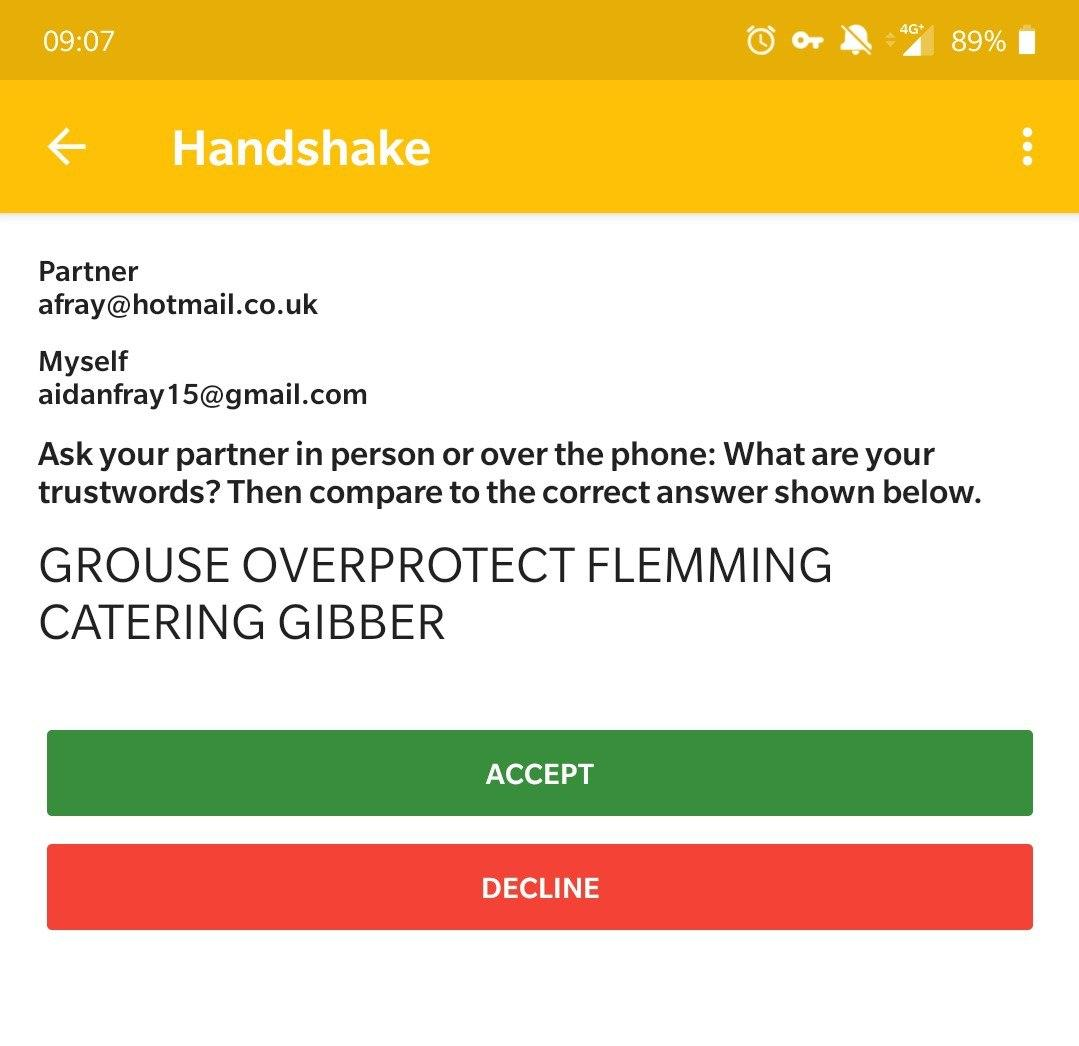
\includegraphics[scale=0.15]{trustwords/trustword_handshake.jpg}
    \caption{Trustword fingerprint verification}
    \label{fig:trustwords}
\end{wrapfigure}

\pep deals with the threat of MiTM attacks by having users compare the respective key fingerprints encoded as a set of words. Figure \ref{fig:trustwords} shows the \pep Android implementation of Trustwords. The users then authenticate the words on an OOB (Out of Band) channel such as a phone call or in-person communication. If both users decide the words match they will accept or decline respectively.

The unique aspect of TrustWords is its mapping of a single word to 16-bits. In comparison to other literature, this is the highest number of bits-per-word seen. Full mappings (no duplication of words) would, therefore, require $2^{16}$ words in the dictionary where arguably the dictionary size is higher than most users' vocabulary. This deviation from the norm has not been currently backed up by research. 

\begin{wrapfigure}{l}{5cm}
    \centering
    \begin{BVerbatim}
    [...]
52127 ZYGOTE
52128 ZYGOTIC
52129 ZYMURGY
52130 AACHEN
52131 AARDVARK
52132 AAREN
    [...]
    \end{BVerbatim}
    \caption{Re-mapping position in Trustword dictionary}
    \label{fig:remap}
\end{wrapfigure}

Alongside the abnormally high number of words the design choice to exclude slang and profanities from the English Trustword dictionary requires dual-mapping of a section of words. Approximately 13633/65536 (20.8\%) of words are re-mapped in the dictionary leaving 51903 unique words. The re-mapping is also done on a loop with it remaining alphabetical. Figure \ref{fig:remap} shows the position in the dictionary where this occurs. This predictability within the dictionary will be explored later in the paper.

Moreover the main RFC documentation still remains in a draft stage and states \textit{``It is for further study, what minimal number of words (or entropy) should be required.''}. These aspects clearly highlight on a gap in the current literature.

\subsubsection*{Topic conclusion}

In conclusion to this topic, the current research has primarily focused on the research and creation of visual representations. Research for textual fingerprints is fragmented and incomplete with work Juola and Zimmermann 
\cite{juola1996whole} and M. Goodrich \textit{et al.}\cite{goodrich2006loud} providing meaningful research to build upon in terms of word a sentence based encodings. The fragmentation of this research leaves room for further work into this topic area. Alongside this, findings from the previous sections research shows that human language based encodings provided the best usability and, therefore, should be a target for further research looking to improve upon their security and usability.

\subsection{Attacks on encoding schemes}
This area of research studies ways to physically execute attacks on fingerprint encoding schemes. This differs from previously examined work due to papers discussing the performance and fallibility of encoding schemes simulated the attack without consideration for how the attack would be performed. Research in this area is scant, with lots of research attention being directed towards the security of Man-in-the-Middle (MITM) attacks and not the encoding schemes themselves.

Research in 2002 by \textbf{Konrad Rieck}\cite{rieck2002fuzzy} is the first formalisation of attacks on fingerprint representations. The paper titled \textit{``Fuzzy Fingerprints Attacking Vulnerabilities in the Human Brain''}
aimed to look into ways users check hexadecimal encoded OpenSSH fingerprint representations. The author created an elegant way to `weight' more important chunks of the digest. The bytes furthest to the right and left of the digests provided the highest weight. The weight was the smallest in the centre of the digest. This provides a way to score digests and determine the best partial collisions found. For example with the target fingerprint: \verb|9F23| a partial match \verb|9313| is given a score of 45\% even though only two characters were matching. This is due to the weightings.

The paper contains an implementation with a ``1.2GHz CPU'' being able to obtain 130,000 H/s (With MD5). In comparison to this, a mid-range Intel i5-3320M CPU can today obtain 111,700,000 MD5 H/s. This shows that the results obtained from the paper are significantly outdated. However, even with the low hash rate, the author was able to obtain some promising results. Figure~\ref{ref:fuzz} contains the best example used.

\begin{figure}[!h]
    \begin{center}
        \verb|TARGET: d6:b7:df:31:aa:55:d2:56:9b:32:71:61:24:08:44:87|
        \verb|MATCH:  d6:b7:8f:a6:fa:21:0c:0d:7d:0a:fb:9d:30:90:4a:87|
    \end{center}
    \caption{Best match obtained after a few minutes of hashing}
    \label{ref:fuzz}
\end{figure}

Overall the paper shows an interesting way to create partial fingerprint matches but is not quantified by any empirical evidence gathered on real world users. This, therefore, highlights on gaps in the coverage of this literature.

The only other relevant research on this topic is the work by \textbf{M Shirvanian \textit{et al.}}\cite{shirvanian2014wiretapping} 
and their paper \textit{``Wiretapping via Mimicry: Short 
Voice Imitation Man-in-the-Middle Attacks on Crypto 
Phones''}. Further research in the area of ``human voice impersonation'' has received lots of attention \cite{mukhopadhyay2015all}\cite{chen2017you}\cite{wu2015spoofing}. This paper was chosen over other alternatives due to is specific use of encoding schemes in its evaluation.

In this paper, the authors develop a way to 
impersonate users when authenticating 
Short-authentication-Strings (SAS) in pairing of 
Crypto-phones. To achieve this impersonating they propose 
two methods: ``Short voice reordering attack'' where an 
arbitrary SAS string is recreated by re-ordering snipped 
obtained from eavesdropping a previous connection
and ``Short voice morphing attacks'' whereby the use of 
previously eavesdropped audio snippets the attacker can
morph their own voice to match that of the victim. With 
these methods, they aimed to attack encodings of Numbers, 
PGP word list (previously discussed work by Juola and 
Zimmermann \cite{juola1996whole}) and MadLib (M. Goodrich 
\textit{et al.}\cite{goodrich2006loud} work also 
previously discussed). The effectiveness of these attacks 
were evaluated with a study involving 30 participants.

Results from the paper show the effectiveness of these 
methods. Compared to the baseline of the attacker's voice 
replacing the victim where this performed with a 
$\sim$18\% success rate. Morphing gained an 
overall success rate of 50.58\% and Reordering a very 
impressive 78.23\% success rate. Showing that these 
attacks provide an improvement on top of the naive implementation.

One of the biggest limitations addressed by the authors 
was the reduction in success rates as the size of the 
authentication string grew. The morphing and reordering 
attacks become increasingly ineffective as the user has 
more time to detect imperfections. This is not quantified by 
the author and the extent of this degradation is never 
empirically discussed. Therefore, the results from this 
study are only effective and applicable in a SAS context.

\subsubsection*{Topic Conclusion}
Overall the literature for this subtopic remains sparse and incomplete. Further suggested work could look into the feasibility of generating partial collisions for all textual representations alongside quantified effectiveness on users. With the possibility to concentrate on a few selected implementations. The work would aim to focus on the various physical methods used and their feasibility. This is one area the previous literature has failed to cover and has only theoretically quantified attacker strength without consideration for the actual real-world cost of these attacks.

\section{Overall Summary}
In summary of the literature gaps areas discovered; encoding scheme performance requires further work in the performance of all graphical schemes to back up the results made by other work. Furthermore, there is a gap with the assessment of encoding schemes in the context of "remote-vs-proximity" first proposed by M. Shirvanian et al. as it would arguably provide a better simulation of real world scenarios.

In the context of human attributes and the way they alter the performance of the schemes; further research is required into how the fluency of languages affects authentication ceremony. This is a continuation of the initial work by Hsiao et al and could allow the creation of schemes that are better suited to certain languages.
Alongside this, there is a research gap in the investigation of how mental impairments affect the performance. This is useful due to the number of potential users being affected due to systems not being designed with them in mind. For example, 7\% of the population has been identified as having dyslexic tendencies\cite{peterson2012developmental}. This means with a UK population of around 63,000,000\footnote{From the 2011 Census collated by the Office for National Statistics}  4,410,000 people could benefit from encoding schemes including dyslexic oriented benefits. This is also only one of many visual impairments that could affect a scheme's performance, thus further contributing to the substantial affect further work could have on this area.

Other possible large areas for consideration is the lacks of direct consideration for attack strength when assessing the vulnerability of encoding schemes. Issues included the wide range of attack strength ($2^{28}$ - $2^{242}$) and the lack of consideration at all from certain papers. This alongside the complete lack of computation and storage complexity considerations means this is a prime area for further research as it would improve the applicability of results.

The final major research gap identified is the lack of justification into the newly created \pep Trustwords. Abnormal design choices (16-bit per word) and its recent creation makes it another area for a wide variety of further research. This is also combined with the conclusive results from the literature on the effectiveness of language based encodings such as words. This would suggest that research into the improvement of Trustword encoding would be highly beneficial.